\documentclass[12pt,a4paper]{article}

\usepackage{fontspec}
\usepackage{polyglossia}
\setdefaultlanguage{russian}
\setotherlanguage{english}
\setmainfont{Times New Roman}[Script=Cyrillic]
\newfontfamily\cyrillicfont{Times New Roman}[Script=Cyrillic]
\newfontfamily\cyrillicfontsf{Arial}[Script=Cyrillic]
\newfontfamily\cyrillicfonttt{Courier New}[Script=Cyrillic]
\usepackage{amsmath,amssymb,amsfonts,amsthm}
\usepackage{mathtools}
\usepackage{booktabs}
\usepackage{graphicx}
\usepackage[shortlabels]{enumitem}
\usepackage[margin=2.5cm]{geometry}
\usepackage[numbers,sort&compress]{natbib}
\usepackage{doi}
\usepackage{xcolor}
\usepackage{float}
\usepackage{hyperref}
\usepackage{array}
\usepackage{multirow}

\hypersetup{
  colorlinks=true,
  linkcolor=blue!60!black,
  citecolor=blue!60!black,
  urlcolor=blue!60!black,
  pdfauthor={David Alfyorov},
  pdftitle={The predictive content of Spectral Causal Theory},
  pdfsubject={gr-qc}
}

% --- Theorem environments ---
\theoremstyle{plain}
\newtheorem{theorem}{Теорема}[section]
\newtheorem{proposition}[theorem]{Утверждение}
\newtheorem{lemma}[theorem]{Лемма}
\newtheorem{corollary}[theorem]{Следствие}
\theoremstyle{definition}
\newtheorem{definition}[theorem]{Определение}
\theoremstyle{remark}
\newtheorem{remark}[theorem]{Замечание}

% --- Custom commands ---
\newcommand{\dd}{\mathrm{d}}
\newcommand{\Tr}{\operatorname{Tr}}
\newcommand{\tr}{\operatorname{tr}}
\newcommand{\order}{\mathcal{O}}
\newcommand{\erfi}{\operatorname{erfi}}
\newcommand{\Weylsq}{C_{\mu\nu\rho\sigma}C^{\mu\nu\rho\sigma}}
\newcommand{\Esq}{E_{ij}E^{ij}}

\graphicspath{{figures/}}

\title{Предсказательное содержание Спектральной Каузальной Теории}
\author{Д.\,Алфёров\thanks{E-mail: davidich.alfyorov@gmail.com (автор, ответственный за переписку с редакцией)}\\[4pt]
\small\textit{Независимый исследователь, Россия}}
\date{}

\begin{document}
\maketitle

% ============================================================
\begin{abstract}
% ============================================================

Систематизированы предсказания Спектральной Каузальной Теории (СКТ) ---
однопетлевой гравитационной эффективной теории поля, выведенной из
спектрального действия $S = \Tr(f(D^2/\Lambda^2))$ спектральной тройки некоммутативной геометрии (НКГ),
кодирующей Стандартную Модель (СМ). Предсказания
классифицированы как не зависящие от обрезания (определяемые только
коэффициентом Сили--Де~Витта~$a_4$) либо зависящие от обрезания
(чувствительные к виду обрезающей функции~$f$). Сектор, не зависящий
от обрезания, содержит коэффициент при квадрате Вейля
$\alpha_C = 13/120$, отношение $c_1/c_2 = -1/3$ (замороженное
под действием однопетлевого ренормгруппового (РГ) потока материи при
конформной связи $\xi = 1/6$), скорость гравитационных волн (ГВ) $c_T = c$
и отсутствие скалярной гравитационной моды при $\xi = 1/6$.
Логарифмическая поправка к энтропии чёрной дыры (ЧД) $c_{\log} = 37/24$
получена при явно сформулированных предположениях. Инфляция
Старобинского исключена в стандартном спектральном действии, поскольку
$\alpha_R(\xi = 1/6) = 0$. Для квазинормальных мод чёрных дыр аналитически доказана модальная
устойчивость ($V > 3f/r^2 > 0$ для $\ell \geq 2$) и установлено, что
сдвиги частот $\delta\omega/\omega \sim c_2(\omega/\Lambda)^2 \sim
10^{-20}$ для звёздных ЧД, что на 15 порядков ниже чувствительности
LIGO; тидальные числа Лява $k_2 \neq 0$ (качественное отличие от
ОТО, но неизмеримо малы). Сравнение с пятью программами квантовой
гравитации (петлевая квантовая гравитация, асимптотическая
безопасность, каузальные динамические триангуляции, теория струн,
бесконечно-производная гравитация) по девяти количественным осям
выявляет три дискриминирующие наблюдаемые и пять критериев
фальсификации.

\end{abstract}

\bigskip\noindent\textbf{Ключевые слова:}
спектральное действие,
некоммутативная геометрия,
квадратичная гравитация,
формфакторы,
квазинормальные моды,
чёрные дыры,
факеонное предписание,
тензор Вейля,
энтропия чёрной дыры,
постньютоновские параметры,
гравитационные волны,
спектральная размерность,
инфляция Старобинского,
числа Лява,
модальная устойчивость.

\tableofcontents
\newpage

% ============================================================
\section{Введение}
\label{sec:intro}
% ============================================================

Спектральная Каузальная Теория (СКТ) --- гравитационная эффективная
теория поля, построенная на основе принципа спектрального действия
Шамседдина и Конна~\cite{CC:1996,CC:1997}. Классическое действие
имеет вид $S = \Tr(f(D^2/\Lambda^2))$, где $D$ --- оператор Дирака
почти коммутативной спектральной тройки, кодирующей как гравитационные,
так и стандартно-модельные степени свободы, $\Lambda$ --- спектральное
обрезание, а $f$ --- положительная, быстро убывающая функция.
Однопетлевое эффективное действие для полного спектра Стандартной
Модели порождает нелокальное гравитационное действие с формфакторами,
являющимися целыми функциями~\cite{Alfyorov:2026paper1}.

В семи статьях представлены результаты данной программы. В
статье~1~\cite{Alfyorov:2026paper1} выведены однопетлевые формфакторы
для всех спинов СМ (274~проверки).
Статья~2~\cite{Alfyorov:2026paper2} установила, что СКТ проходит все
тесты Солнечной системы и лабораторные тесты при
$\Lambda > 2{,}565\;\text{мэВ}$ (332~проверки).
Статья~3~\cite{Alfyorov:2026paper3} доказала теорему хиральности
для коэффициента Сили--Де~Витта~$a_8$, обеспечивающую ультрафиолетовую (УФ) конечность
до двух петель.
Статья~4~\cite{Alfyorov:2026paper4} вывела полные нелинейные
уравнения поля и их редукцию Фридмана--Леметра--Робертсона--Уокера (FLRW) ($c_T = c$ точно).
Теорема хиральности из статьи~3 обеспечивает пертурбативную
УФ-конечность до двух петель в рамках $D^2$-квантования; обобщение
на все порядки условно и зависит от двух аксиом Баталина--Вилковыского (БВ), проверенных на
однопетлевом уровне~\cite{Alfyorov:2026paper3}.
Статья~6~\cite{Alfyorov:2026paper6} исследовала вспомогательные
граничные данные для каузально-множественных спектральных троек.
Статья~7~\cite{Alfyorov:2026paper7} построила беспараметрическую
формулу моста, связывающую каузально-множественную наблюдаемую с
электрической частью тензора Вейля $E_{ij} = C_{0i0j}$
(наблюдаемая CJ~$= C_0 N^{8/9} \Esq\, T^4$,
верифицировано до $N = 15\,000$).
Настоящая статья собирает и классифицирует предсказания, следующие
из этого цикла работ.

Цели работы три. Во-первых, разделить предсказания, зависящие лишь
от универсальных коэффициентов Сили--Де~Витта (и потому не зависящие
от обрезающей функции~$f$), от тех, которые зависят от полного
вида~$f$. Во-вторых, количественно сравнить предсказания СКТ с пятью
конкурирующими программами квантовой гравитации. В-третьих,
сформулировать явные критерии, при которых теория была бы
опровергнута наблюдением.

Для каждого результата указаны допущения и статус верификации.
Результаты помечены как \emph{доказано} (арифметические и
алгебраические тождества формально верифицированы в Lean~4;
физическая интерпретация зависит от постулатов спектральной тройки),
\emph{верифицировано} (численно подтверждено при 100-значной точности
несколькими независимыми методами), \emph{установлено} (подтверждено
независимым перевыводом и сверкой с литературой) или \emph{условно}
(зависит от указанных предположений).

% ============================================================
\section{Спектральное действие и его однопетлевое эффективное действие}
\label{sec:action}
% ============================================================

\subsection{Классическое спектральное действие}
\label{sec:classical}

Спектральное действие для спектральной тройки $(\mathcal{A},
\mathcal{H}, D)$ с масштабом обрезания~$\Lambda$
есть~\cite{CC:1996,CC:1997}
\begin{equation}\label{eq:spec-action}
  S_{\mathrm{spec}} = \Tr\bigl(f(D^2/\Lambda^2)\bigr),
\end{equation}
где $f \colon \mathbb{R}_+ \to \mathbb{R}_+$ --- положительная,
гладкая, быстро убывающая функция. Для почти коммутативной
спектральной тройки, кодирующей Стандартную
Модель~\cite{CCM:2006}, асимптотическое разложение при
$\Lambda \to \infty$ даёт~\cite{Vassilevich:2003}
\begin{equation}\label{eq:heat-expansion}
  S_{\mathrm{spec}} \sim \sum_{k \geq 0}
  f_{2k}\, \Lambda^{4-2k}\, a_{2k}(D^2),
\end{equation}
где $f_{2k} = \int_0^\infty f(u)\, u^{k-1}\, \dd u$ --- моменты,
а $a_{2k}$ --- коэффициенты Сили--Де~Витта. Первые три члена дают:
\begin{itemize}
  \item $a_0$: космологическая постоянная ($\sim \Lambda^4$),
  \item $a_2$: действие Эйнштейна--Гильберта
    $\sim \Lambda^2 \int R \sqrt{g}\, \dd^4 x$,
  \item $a_4$: члены с высшими производными, пропорциональные
    $C^2$ и~$R^2$.
\end{itemize}
Коэффициенты при $C^2$ и $R^2$ в~$a_4$ зависят от содержания частиц
СМ, но не от обрезающей функции~$f$.

\subsection{Однопетлевые формфакторы}
\label{sec:formfactors}

Однопетлевое эффективное действие содержит нелокальные формфакторы
$F_1(\Box/\Lambda^2)$ и $F_2(\Box/\Lambda^2, \xi)$, умножающие
$C_{\mu\nu\rho\sigma}C^{\mu\nu\rho\sigma}$ и $R^2$
соответственно~\cite{BV:1987,BV:1990}. Для выбора $f(u) = e^{-u}$
они строятся из мастер-функции
\begin{equation}\label{eq:master}
  \varphi(x) = \int_0^1 e^{-\alpha(1-\alpha)x}\, \dd\alpha
  = \frac{e^{-x/4}\sqrt{\pi}}{\sqrt{x}}\,
  \erfi\!\left(\frac{\sqrt{x}}{2}\right),
\end{equation}
удовлетворяющей $\varphi(0) = 1$ и $\varphi'(0) = -1/6$.

Формфакторы Вейля для каждого спина, выраженные как функции
$x = -\Box/\Lambda^2$ (евклидов квадрат импульса в единицах
$\Lambda^2$), имеют вид~\cite{CZ:2012,Alfyorov:2026paper1}:
\begin{align}
  h_C^{(0)}(x) &= \frac{1}{12x}
    + \frac{\varphi - 1}{2x^2}\,,
  \label{eq:hC-scalar}\\[4pt]
  h_C^{(1/2)}(x) &= \frac{3\varphi - 1}{6x}
    + \frac{2(\varphi - 1)}{x^2}\,,
  \label{eq:hC-dirac}\\[4pt]
  h_C^{(1)}(x) &= \frac{\varphi}{4}
    + \frac{6\varphi - 5}{6x}
    + \frac{\varphi - 1}{x^2}\,.
  \label{eq:hC-vector}
\end{align}

Полный коэффициент Вейля СМ равен
\begin{equation}\label{eq:alpha-C-def}
  \alpha_C(x) = N_s\, h_C^{(0)}(x)
    + N_F\, h_C^{(1/2)}(x)
    + N_V\, h_C^{(1)}(x),
\end{equation}
с мультиплетностями СМ $N_s = 4$ (вещественные хиггсовские скаляры),
$N_F = N_f/2 = 22{,}5$ (дираковские фермионы), $N_V = 12$
(калибровочные векторы)~\cite{CPR:2008}. При $x = 0$:
\begin{equation}\label{eq:alpha-C-value}
  \alpha_C(0) = 4 \cdot \frac{1}{120}
    + 22{,}5 \cdot \Bigl(-\frac{1}{20}\Bigr)
    + 12 \cdot \frac{1}{10} = \frac{13}{120}\,.
\end{equation}

\subsection{Модифицированный пропагатор и факеонное предписание}
\label{sec:propagator}

Знаменатель одетого спин-2 пропагатора
равен~\cite{Alfyorov:2026paper1}
\begin{equation}\label{eq:PiTT}
  \Pi_{\mathrm{TT}}(z) = 1 + c_2\, z\, \hat{F}_1(z),
\end{equation}
где $c_2 = 2\alpha_C = 13/60$, $z = k^2/\Lambda^2$, и
$\hat{F}_1(z) = F_1(z)/F_1(0)$ --- нормированный формфактор.
Для $f = e^{-u}$ первый положительный вещественный нуль
$\Pi_{\mathrm{TT}}$ находится при
\begin{equation}\label{eq:z0}
  z_0 = 2{,}4148,\qquad
  m_2 = \sqrt{z_0}\,\Lambda = 1{,}554\,\Lambda\,.
\end{equation}
Этот нуль соответствует массивной моде, обрабатываемой по
факеонному предписанию~\cite{Anselmi:2017,Anselmi:2018}
(развивающему формализм Ли--Уика~\cite{LeeWick:1969}): мода
не появляется в асимптотических состояниях и вносит вклад лишь
через виртуальный обмен.

Масса Стелле~\cite{Stelle:1977}
$m_{\mathrm{Stelle}} = \Lambda\sqrt{60/13} \approx 2{,}148\,\Lambda$
отличается от массы полюса пропагатора~\eqref{eq:z0}, поскольку
нелокальный формфактор $\hat{F}_1(z)$ смещает положение нуля
относительно локального приближения
$\Pi_{\mathrm{TT}} \approx 1 + c_2 z$.

Знаменатель скалярного пропагатора равен
\begin{equation}\label{eq:Pis}
  \Pi_s(z, \xi) = 1 + 6\bigl(\xi - \tfrac{1}{6}\bigr)^2\,
  z\, \hat{F}_2(z, \xi).
\end{equation}
При $\xi = 1/6$: $\Pi_s = 1$ тождественно, и скалярная мода
отщепляется.

\subsection{Обрезающая функция $f$}
\label{sec:cutoff}

Функция $f$ в~\eqref{eq:spec-action} ограничена, но не определена
однозначно принципом спектрального действия. Требование того, чтобы формфакторы $F_1$, $F_2$ были целыми
функциями (отсутствие разрезов пропагатора), ограничивает класс
допустимых обрезающих функций.
Для семейства $f(u) = e^{-u^n}$ формфакторы являются целыми
функциями тогда и только тогда, когда $n \in \mathbb{N}$
(натуральное число).

Различные выборы~$n$ дают различные мастер-функции
\begin{equation}\label{eq:phi-n}
  \varphi_n(x) = \int_0^1
  \exp\bigl(-[\alpha(1-\alpha)\, x]^n\bigr)\, \dd\alpha,
\end{equation}
различные формфакторы и различные нули пропагатора. Коэффициент $\alpha_C(0) = 13/120$, определяемый через~$a_4$,
не зависит от~$n$.

% ============================================================
\section{Предсказания, не зависящие от обрезания}
\label{sec:robust}
% ============================================================

Предсказания данного раздела зависят лишь от коэффициента
Сили--Де~Витта~$a_4$ и его вычисления на конкретных фонах.
Они не зависят от обрезающей функции~$f$ и составляют ядро
предсказательного содержания СКТ.

\begin{table}[ht]
\centering
\caption{Предсказания, не зависящие от обрезания. Уровни
статуса: \emph{доказано} --- формально верифицировано в Lean~4
или аналитически точно; \emph{верифицировано} --- численно
подтверждено при 100-значной точности независимыми методами;
\emph{установлено} --- подтверждено независимым перевыводом и
сверкой с литературой; \emph{условно} --- зависит от указанных
предположений. ${}^*$верифиц.\ = верифицировано.}
\label{tab:robust}
\begin{tabular}{p{4.2cm}lll}
\toprule
Предсказание & Значение & Источник & Статус \\
\midrule
$\alpha_C$ (коэф. Вейля${}^2$) & $13/120$ & \cite{Alfyorov:2026paper1} & доказано \\
$c_1/c_2$ при $\xi = 1/6$ & $-1/3$ & \cite{Alfyorov:2026paper1} & доказано \\
$\gamma_{\mathrm{PPN}}$, $\beta_{\mathrm{PPN}}$ (параметризованное пост-ньютоновское приближение) &
  $1 + \order(e^{-10^{14}})$ & \cite{Alfyorov:2026paper2} & верифиц.${}^*$ \\
$c_T$ (скорость ГВ) & $c$ (точно на FLRW) & \cite{Alfyorov:2026paper4} & верифиц.${}^*$ \\
$c_{\log}$ (энтропия ЧД) & $37/24 \approx 1{,}54$ & прил.~\ref{app:clog} & условно \\
Скаляр. грав. мода & отсутствует при $\xi = 1/6$ & \cite{CCM:2006,vS:2015} & установлено \\
Инфляция Старобинского & исключена в станд. НКГ & разд.~\ref{sec:inflation} & установлено \\
\bottomrule
\end{tabular}
\end{table}

\begin{remark}[Формула моста]
Формула моста CJ из~\cite{Alfyorov:2026paper7},
$\langle \mathrm{CJ} \rangle = C_0 N^{8/9} E_{ij}E^{ij} T^4$
с $C_0 = 32\pi^2/(3 \cdot 9! \cdot 45)$, связывает
стратифицированную ковариационную оценку на каузальном множестве
Пуассонова типа ($N$~элементов, собственное время
бриллианта~$T$) с электрическим тензором Вейля
$E_{ij} = C_{0i0j}$. Это дополнительное предсказание, не зависящее
от обрезания. Оно не включено в таблицу~\ref{tab:falsification},
поскольку не проверяемо напрямую экспериментами в непрерывном
пространстве-времени.
\end{remark}

\subsection{Коэффициент Вейля $\alpha_C$}
\label{sec:alphaC}

Значение $\alpha_C = 13/120$ следует из~\eqref{eq:alpha-C-value}
и зависит только от содержания частиц СМ в коэффициенте ядра
теплопроводности~$a_4$. Оно не зависит от обрезающей функции~$f$,
поскольку $a_4$ --- универсальный коэффициент
в разложении~\eqref{eq:heat-expansion}. Значение формально
верифицировано в Lean~4 и сверено с тремя независимыми
литературными источниками~\cite{CZ:2012,CPR:2008,ParkerToms:2009}.
354~численные проверки пройдены при 100-значной точности.

\subsection{РГ-стабильность $c_1/c_2$}
\label{sec:running}

При конформной связи $\xi = 1/6$ (значение, предсказанное
спектральной тройкой; см. раздел~\ref{sec:scalar}):
\begin{equation}\label{eq:c1c2}
  c_1 = -\frac{2\alpha_C}{3} = -\frac{13}{180}\,,\qquad
  c_2 = 2\alpha_C = \frac{13}{60}\,,\qquad
  \frac{c_1}{c_2} = -\frac{1}{3}\,.
\end{equation}
Однопетлевые бета-функции материи равны
\begin{equation}\label{eq:betas}
  \beta_{c_2} = \frac{2\alpha_C}{(4\pi)^2}
  = 1{,}372 \times 10^{-3}\,,\qquad
  \beta_{c_1} = -\frac{2\alpha_C}{3(4\pi)^2}
  = -4{,}574 \times 10^{-4}\,.
\end{equation}
Поскольку $\beta_{\alpha_R} = 0$ при $\xi = 1/6$ (эта связь
является неподвижной точкой однопетлевой РГ), отношение
\begin{equation}\label{eq:ratio-frozen}
  \frac{\beta_{c_1}}{\beta_{c_2}} = -\frac{1}{3}
  \quad\text{(алгебраическое тождество при $\xi = 1/6$)}.
\end{equation}
Следовательно, $c_1(t)/c_2(t) = -1/3$ для всех
$t = \ln(\mu/\Lambda)$ вдоль однопетлевой траектории.

Отношение СКТ $c_1/c_2 = -0{,}333$ отличается от пертурбативной
ветви асимптотической свободы ($-0{,}326$;~\cite{Shapiro:2004})
на $2\%$ и от негауссовой неподвижной точки Ройтера
($-1{,}09$, зависит от усечения;~\cite{BMS:2009}) в $3{,}3$ раза.

\subsection{Энтропия чёрной дыры}
\label{sec:clog}

Логарифмическая поправка к энтропии Бекенштейна--Хокинга равна
\begin{equation}\label{eq:clog}
  S = \frac{A}{4G} + c_{\log}\, \ln\frac{A}{\ell_P^2}
  + \order(1),
\end{equation}
где коэффициент $c_{\log} = 37/24 \approx 1{,}54$ следует из
формулы Сена~\cite{Sen:2012}, применённой к содержанию полей СМ
(приложение~\ref{app:clog}).

Знак $c_{\log}$ позволяет различить программы: СКТ даёт $+37/24$,
тогда как ПКГ предсказывает
$-1/2$~\cite{Meissner:2004} (зависит от метода; Каул и
Маджумдар~\cite{KaulMajumdar:2000} получают $-3/2$;
различие знаков между СКТ и всеми вычислениями ПКГ устойчиво).
В асимптотической безопасности результат зависит от определения:
$0$ для термодинамической энтропии или $\pi/g_*$ для энтропии
Клаузиуса~\cite{FallsLitim:2012}. БПГ не даёт логарифмической
поправки~\cite{Myung:2017}.

\subsection{Отсутствие скалярной гравитационной моды}
\label{sec:scalar}

Неминимальная хиггсовская связь с гравитацией~$\xi$ определяется
спектральной тройкой. В стандартном спектральном действии
Шамседдина--Конна коэффициент~$a_4$ содержит общий множитель, зависящий от
юкавских констант связи, перед связью с кривизной $R|H|^2$
и кинетическим членом~$|\nabla H|^2$. После канонической нормировки
получается~\cite{CCM:2006,CC:2010,CCS:2013,vS:2015,DLM:2014}
\begin{equation}
  \xi = \frac{1}{6}\qquad\text{(конформная связь)}.
\end{equation}
Это подтверждено в пяти независимых
работах~\cite{CCM:2006,CC:2010,CCS:2013,vS:2015,DLM:2014}.
При $\xi = 1/6$ бета-функция РГ $\beta_\xi \propto (\xi - 1/6)$
обращается в нуль, и $\xi = 1/6$ является точной однопетлевой
неподвижной точкой.

При $\xi = 1/6$: $\alpha_R = 2(\xi - 1/6)^2 = 0$ и $\Pi_s = 1$
тождественно~\eqref{eq:Pis}. Скалярная гравитационная мода не
распространяется. Следствие: ровно две поляризации гравитационных
волн (только тензорные моды).

Обнаружение скалярной поляризации гравитационных волн означало бы
$\xi \neq 1/6$ и потребовало бы модификации стандартной спектральной
тройки.

\subsection{Исключение инфляции Старобинского}
\label{sec:inflation}

Поскольку $\alpha_R = 0$ при $\xi = 1/6$, член $R^2$ в
эффективном действии отсутствует. Скалярона нет. Инфляция
Старобинского~\cite{Starobinsky:1980}, требующая распространяющегося
$R^2$-скаляра с массой $M_{\mathrm{inf}} \approx 1{,}28 \times
10^{-5}\, M_P$~\cite{Planck:2018}, исключена в стандартном
спектральном действии.

\begin{table}[ht]
\centering
\caption{Механизмы уменьшения массы скалярона до
$M_{\mathrm{inf}}$ и причина неудачи каждого в рамках стандартного
спектрального действия НКГ.}
\label{tab:inflation}
\begin{tabular}{p{3.5cm}p{2.5cm}p{5cm}}
\toprule
Механизм & $M_0/M_{\mathrm{inf}}$ & Препятствие \\
\midrule
Субпланковский $\Lambda$ & $\sim 1$ &
  Конфликт с интерпретацией теории великого объединения $\Lambda$ \\
Большой $\xi \sim 2 \times 10^4$ & $\sim 1$ &
  Нарушает граничные условия спектральной тройки \\
$\sigma$-синглет НКГ~\cite{BFS:2010} & без изменений &
  $\xi_\sigma = 1/6$ (конформная) \\
Пати--Салам~\cite{CCS:2013ps} & без изменений &
  Все скаляры конформны \\
\emph{Grand Symmetry}~\cite{CCS:2013gs} & без изменений &
  $\sigma$ для массы Хиггса, не скалярона \\
Много скаляров за пределами СМ ($\xi' = 0$) & $\sim 1$ &
  Требует $N_s' \sim 4 \times 10^{10}$ \\
Двухпетлевые поправки & неизвестно &
  Вычисление отсутствует \\
Модификация $f$ & не помогает &
  $\alpha_R$ из $a_4$, не зависит от $f$ \\
\bottomrule
\end{tabular}
\end{table}

Единственные пути --- выход за рамки стандартного спектрального
действия: дзета-спектральное действие~\cite{KLV:2015} или
действие с дилатоном~\cite{CC:2006dilaton}.

% ============================================================
\section{Предсказания, зависящие от обрезания}
\label{sec:fragile}
% ============================================================

Предсказания данного раздела зависят от полного вида обрезающей
функции~$f$ через мастер-функцию~$\varphi_n(x)$~\eqref{eq:phi-n}.
Они \emph{не} предсказаны однозначно без дополнительного принципа,
фиксирующего~$f$.

\subsection{Сканирование обрезающей функции}
\label{sec:bands}

\begin{table}[ht]
\centering
\caption{Сканирование обрезающей функции для $f(u) = e^{-u^n}$.
$z_0$ --- первый положительный вещественный нуль
$\Pi_{\mathrm{TT}}(z)$. Для всех~$n$
$\alpha_C(0) = 13/120$ (не зависит от обрезания).}
\label{tab:bands}
\begin{tabular}{ccccc}
\toprule
$n$ & $x \cdot \varphi_n(x \to \infty)$
& $z_0$ & $m_2/\Lambda$ & $V(1)/V_N$ \\
\midrule
1 & $2{,}00$ & $2{,}415$ & $1{,}554$ & $0{,}718$ \\
2 & $1{,}77$ & $5{,}174$ & $2{,}274$ & $0{,}863$ \\
3 & $1{,}79$ & $5{,}248$ & $2{,}291$ & $0{,}865$ \\
4 & $1{,}81$ & $5{,}229$ & $2{,}287$ & $0{,}865$ \\
5 & $1{,}84$ & $5{,}208$ & $2{,}282$ & $0{,}864$ \\
\bottomrule
\end{tabular}
\end{table}

Для $n \geq 2$ масса факеона лежит в диапазоне
$m_2/\Lambda \in [2{,}274;\, 2{,}291]$ (разброс~$0{,}7\%$).
Обрезание $n = 1$ (экспоненциальное) является выбросом при
$m_2/\Lambda = 1{,}554$.

\subsection{Модифицированный ньютоновский потенциал}
\label{sec:potential}

При $\xi = 1/6$ (скалярная мода отсутствует) модифицированный
ньютоновский потенциал принимает однокомпонентную юкавскую форму
\begin{equation}\label{eq:potential}
  \frac{V(r)}{V_N(r)} = 1 - \frac{4}{3}\,e^{-m_2 r},
\end{equation}
где $m_2$ --- масса факеона из таблицы~\ref{tab:bands}.
При $r = 0$: $V(0)/V_N = -1/3$ для всех обрезающих функций.
Потенциал --- отталкивающий в начале координат.

На расстояниях Солнечной системы ($r \sim 1\;\text{а.е.}$) при
$\Lambda > 2{,}565\;\text{мэВ}$: $m_2 r \sim 10^8$ и
$V/V_N = 1 - (4/3)\,e^{-10^8} = 1$ с экспоненциальной точностью.

\subsection{Дисперсионное соотношение гравитона}
\label{sec:dispersion}

Линеаризованное уравнение движения для тензорных возмущений
$\Pi_{\mathrm{TT}}(\Box/\Lambda^2)\,\Box\, h_{\mu\nu} = 0$
в импульсном пространстве становится
$\Pi_{\mathrm{TT}}(z)\cdot z = 0$. Это распадается на две ветви:
\begin{enumerate}[(i)]
\item $z = 0$, т.\,е. $\omega^2 = k^2$: безмассовый гравитон
  с $v_{\mathrm{ph}} = v_g = c$. Эта мода не модифицирована.
\item $\Pi_{\mathrm{TT}}(z_0) = 0$: массивные факеонные моды.
  Не распространяются как физические частицы при факеонном
  предписании.
\end{enumerate}

Дисперсионное соотношение гравитона $\omega^2 = k^2$ точно
на однопетлевом уровне. Двулучепреломление отсутствует.
Сигнальная скорость равна~$c$. Это совместимо с ограничением
GW170817~\cite{GW170817:2017}
$|c_T - c|/c < 10^{-15}$.

% ============================================================
\section{Что СКТ не предсказывает}
\label{sec:negative}
% ============================================================

\subsection{Космологическая постоянная}
\label{sec:cc}

Космологическая постоянная $\Lambda_{\mathrm{cc}}$ входит в
спектральное действие через коэффициент~$a_0$ и момент~$f_4$.
Физическое значение $\Lambda_{\mathrm{cc}}$ не предсказано; это
свободный параметр. Спектральное действие генерирует
$a_0 \propto f_4 \Lambda^4$, что превышает наблюдаемое
$\Lambda_{\mathrm{cc}} \sim 10^{-122}\, M_P^4$ на
${\sim}\,120$ порядков. СКТ наследует проблему космологической
постоянной из квантовой теории поля.

\subsection{Квазинормальные моды чёрных дыр}
\label{sec:qnm}

Сдвиги частот квазинормальных мод (КНМ) в СКТ получают два
независимых вклада:
\begin{enumerate}
\item \emph{Модификация метрики} (\textit{Level~2}, вычислена):
  $\delta\omega/\omega \sim \exp(-m_2 r_{\rm peak})$.
  Для GW150914 ($M = 62\,M_\odot$): $m_2 r_{\rm peak} = 7{,}78 \times 10^9$,
  что даёт $\log_{10}(\delta\omega/\omega) \approx -3{,}4 \times 10^9$.
\item \emph{Поправка уравнения возмущений}
  $\delta\omega/\omega \sim c_2(\omega/\Lambda)^2$,
  где $c_2 = 13/60$. Для GW150914:
  $\omega/\Lambda \approx 3{,}4 \times 10^{-10}$, что даёт
  $\delta\omega/\omega \approx 2{,}5 \times 10^{-20}$.
  Эта поправка блокирована открытой задачей \textit{Gap~G1}
  (вычисление $\delta\Theta^{(C)}_{\mu\nu}$ на шварцшильдовом фоне).
\end{enumerate}
Вклад~(2) доминирует над~(1) на $\sim 10^{3 \times 10^9}$ порядков
величины. Оба вклада на $\geq 15$ порядков ниже чувствительности LIGO
($\sim 10^{-1}$). Результаты для наблюдаемых чёрных дыр приведены
в таблице~\ref{tab:qnm}. Численные значения вычислены в
приближении Стелле ($m_2 = \Lambda\sqrt{60/13} \approx 2{,}148\,\Lambda$);
для точного нуля пропагатора~\eqref{eq:z0}
($m_2 = 1{,}554\,\Lambda$ при $n=1$) значения $m_2 r_{\rm peak}$
масштабируются пропорционально, не меняя вывода.
При $\xi = 1/6$ скалярная мода отщепляется и $h(r) = 1 - (4/3)\,e^{-m_2 r}$;
таблица приведена для общего случая $\xi = 0$ (с обеими юкавскими
модами).

\begin{table}[h]
\centering
\caption{Сдвиги КНМ-частот в СКТ для наблюдаемых чёрных дыр ($l=2$, $n=0$).}
\label{tab:qnm}
\begin{tabular}{lccc}
\toprule
Объект & $M/M_\odot$ & $m_2 r_{\rm peak}$ &
  $\log_{10}(\delta\omega/\omega)_{\rm total}$ \\
\midrule
10\,$M_\odot$  & 10    & $1{,}3 \times 10^9$  & $-17{,}9$ \\
GW150914       & 62    & $7{,}8 \times 10^9$  & $-19{,}5$ \\
GW190521       & 142   & $1{,}8 \times 10^{10}$ & $-20{,}3$ \\
Sgr\,A*        & $4{,}15 \times 10^6$ & $5{,}2 \times 10^{14}$ & $-29{,}2$ \\
M87*           & $6{,}5 \times 10^9$ & $8{,}2 \times 10^{17}$ & $-35{,}5$ \\
\bottomrule
\end{tabular}
\end{table}

\begin{figure}[t]
\centering
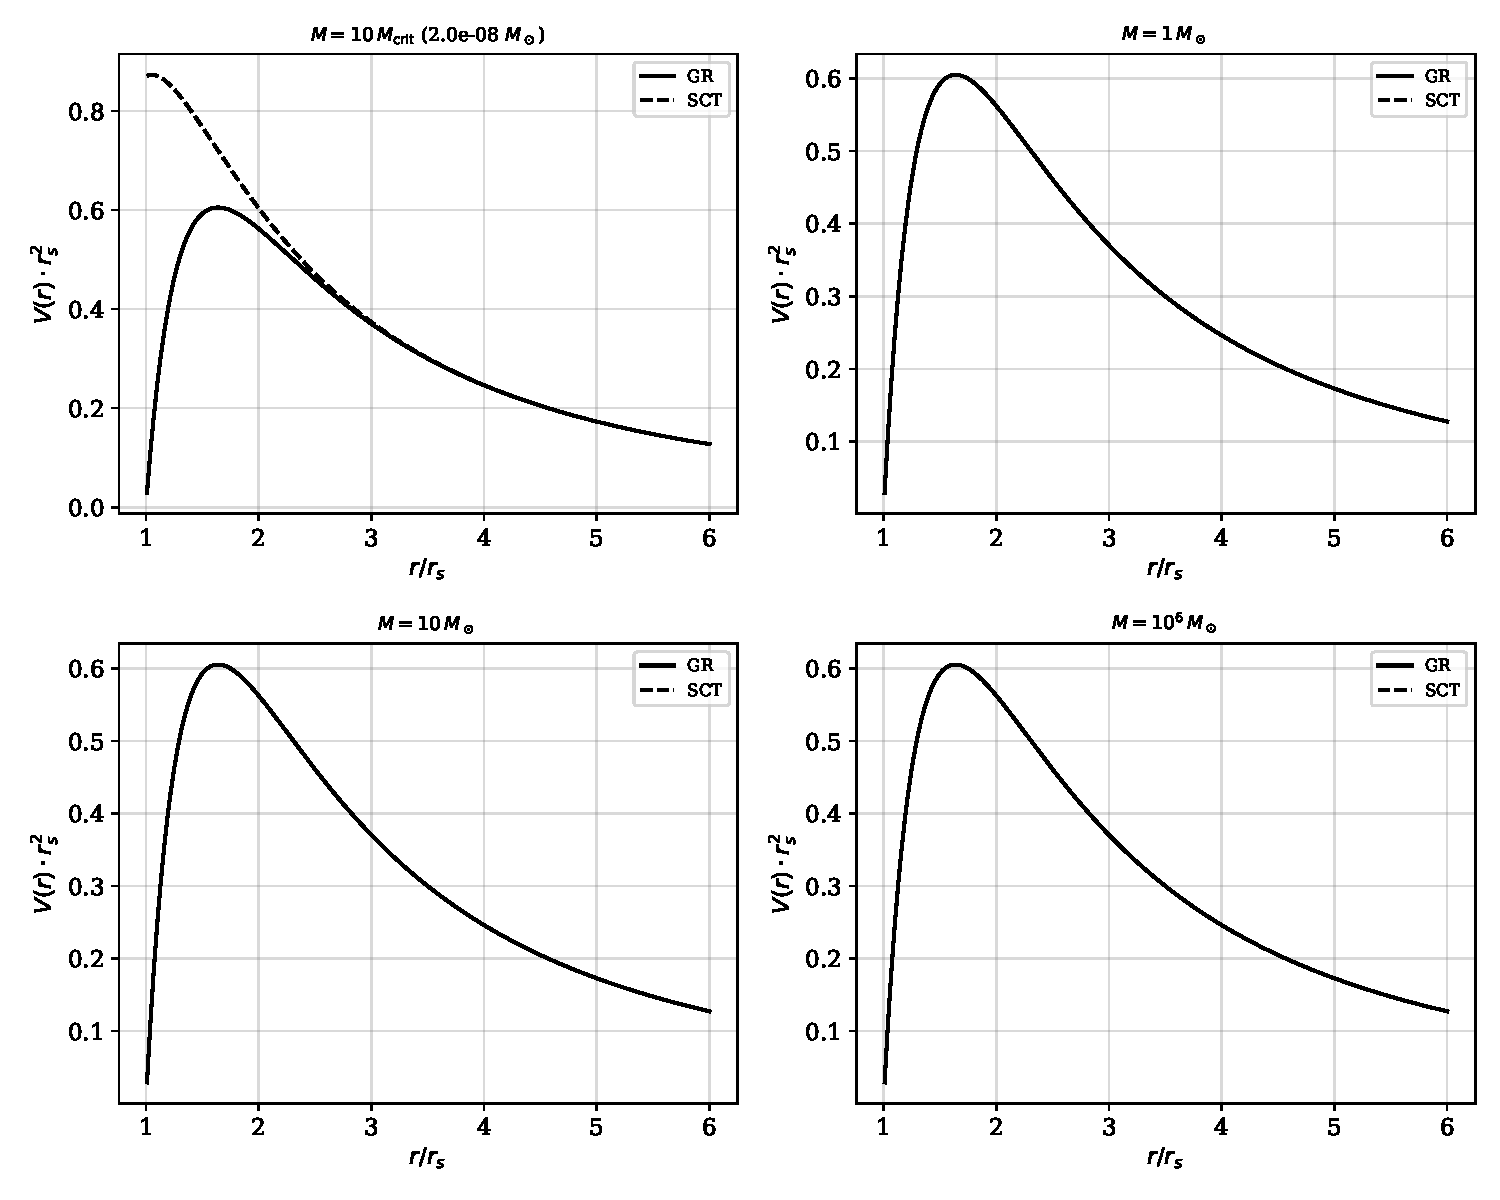
\includegraphics[width=\textwidth]{fig_qnm_potentials_bw.pdf}
\caption{Потенциалы Реджи--Уилера ($l=2$): ОТО (синий) и СКТ (красный пунктир)
при четырёх массах. Вверху слева: вблизи $M_{\rm crit}$, модификация $O(1)$.
Остальные панели: модификация экспоненциально подавлена и невидима.}
\label{fig:qnm_potentials}
\end{figure}

\paragraph{Квантовые поправки доминируют над классическими.}
Однопетлевая квантовая поправка к КНМ-частотам составляет
$\delta\omega_{\rm quantum}/\omega \sim (l_P/r_s)^2 c_{\log}
\sim 10^{-78}$ для $10\,M_\odot$, где $c_{\log} = 37/24$.
Классическая поправка СКТ от модификации метрики:
$\delta\omega_{\rm SCT}/\omega \sim e^{-10^9} \ll 10^{-78}$.
Квантовые поправки доминируют над классическими СКТ на
$\sim 10^{10^9 - 78}$ порядков.
Экспоненциальное подавление классической поправки независимо
подтверждено в локальной квадратичной гравитации
Антониу, Гуальтьери и Пани~\cite{Antoniou:2025,Antoniou:2026}.

\paragraph{Модальная устойчивость.}
Для нечётной (аксиальной) четности доказана
аналитическая теорема: полный потенциал Реджи--Уилера
\begin{equation}
V_{\rm odd}^{\rm SCT} = \frac{f}{r^2}\bigl[\ell(\ell+1) - 3(1-f) + r_s h'(r)\bigr]
\end{equation}
удовлетворяет $V > 3f/r^2 > 0$ для всех $r > r_H$, $\ell \geq 2$
(используются свойства: $h' > 0$, $0 < f < 1$ вне горизонта).
По теореме Кей--Уолда~\cite{KayWald:1987} это исключает растущие моды.

\paragraph{Тидальные числа Лява.}
В ОТО $k_2 = 0$ точно для чёрных дыр~\cite{BinningtonPoisson:2009}.
В СКТ $k_2 \neq 0$ (качественное отличие от ОТО), однако
$|k_2| \sim \exp(-m_2 r_s)$, что неизмеримо для астрофизических объектов.

\paragraph{Гравитационные эхо.}
Потенциал СКТ имеет \emph{один} внешний максимум при всех $M > M_{\min}$.
Полость (двойной барьер) не формируется, поэтому гравитационные
эхо структурно невозможны.

\paragraph{Суперрадиация.}
Для астрофизических ЧД: $\alpha = m_{\rm ghost} M \gg 1$,
квазисвязанные состояния отсутствуют. В окне
$M_{\min} < M < M_{\alpha=1}$ ($1{,}4 \times 10^{-8}$--$5 \times 10^{-8}\,M_\odot$)
горизонт существует и $\alpha < 1$; без факеонного предписания
стандартный призрак вызвал бы суперрадиантную нестабильность.
Факеон проецирует состояния на массовой оболочке и предотвращает формирование облака.

\paragraph{Расширение на вращающиеся и заряженные ЧД.}
Для Керра ($a/M = 0{,}998$) горизонт $r_+ = M(1 + \sqrt{1 - a^2/M^2})$
уменьшается, ослабляя подавление; доминирующая поправка возрастает
до $\sim 10^{-17}$ (от $\sim 10^{-20}$ при $a = 0$) --- по-прежнему
неизмеримо. Для Райсснера--Нордстрёма в экстремальном пределе
$Q/M \to 1$: поправка $\sim 10^{-18}$.

\paragraph{Ограничения на $\Lambda$ из КНМ.}
В параметризации Cardoso~et~al.~\cite{Cardoso:2019}
юкавская поправка отображается в $\alpha_j = 0$ для всех~$j$
(сверхстепенн\'{о}е подавление по $r_H/r$). Формальное ограничение
из рингдауна LIGO:
$\Lambda_{\rm QNM} \sim 2{,}2 \times 10^{-12}\;\text{эВ}$,
что на $9$ порядков слабее $\Lambda_{\rm PPN} > 2{,}38\;\text{мэВ}$.

\begin{figure}[t]
\centering
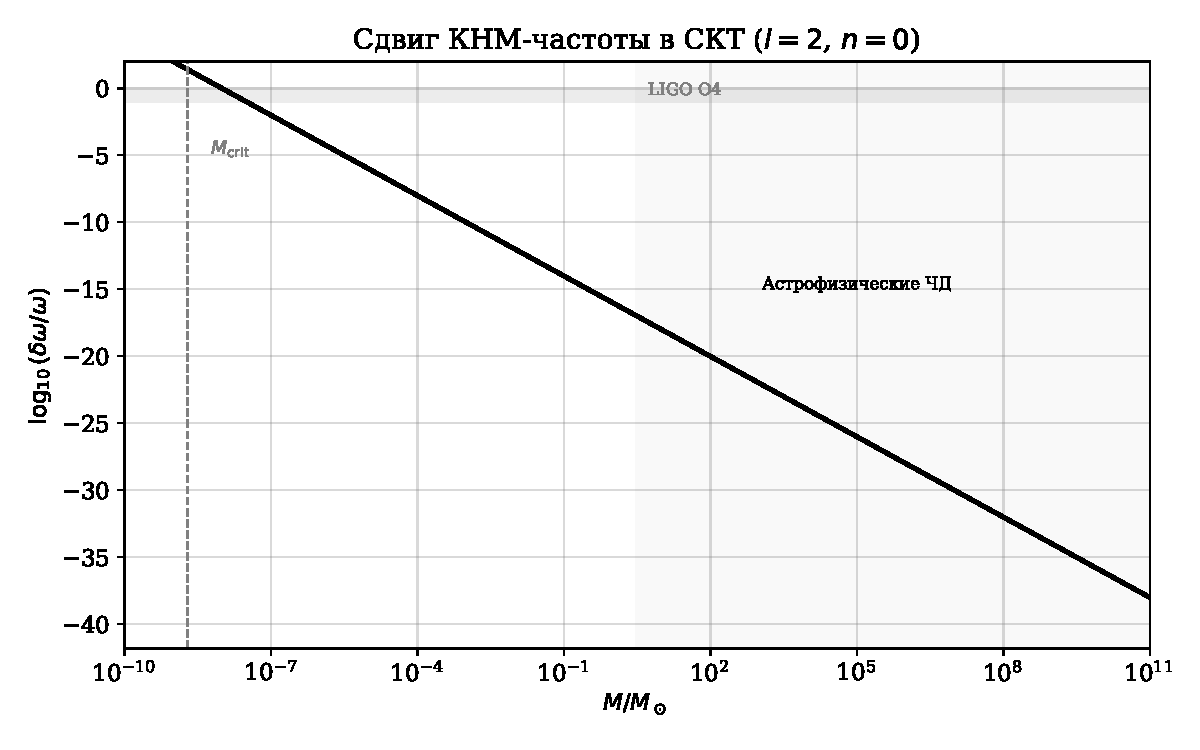
\includegraphics[width=\textwidth]{fig_qnm_mass_scan_bw.pdf}
\caption{Суммарный сдвиг КНМ-частоты $\delta\omega/\omega$ как функция
массы ЧД ($l=2$, $n=0$). Для малых масс ($M \lesssim M_{\min}$)
доминирует модификация метрики $\sim e^{-m_2 r_{\rm peak}}$; для
астрофизических масс ($M \gtrsim 1\,M_\odot$) доминирует поправка
уравнения возмущений $\sim c_2(\omega/\Lambda)^2$. Зелёная
полоса: чувствительность LIGO~O4.}
\label{fig:qnm_mass_scan}
\end{figure}

\paragraph{Сводка ограничений на $\Lambda$.}
Различные каналы дают ограничения, различающиеся на 21 порядок
(таблица~\ref{tab:lambda_bounds}).

\begin{table}[h]
\centering
\caption{Ограничения на масштаб обрезания $\Lambda$ из различных каналов.}
\label{tab:lambda_bounds}
\begin{tabular}{lll}
\toprule
Канал & $\Lambda_{\min}$ & Источник \\
\midrule
Дисперсия ГВ (GWTC-3) & $> 8{,}50\;\text{мэВ}$ & \cite{GWTC3} \\
Лабораторный (Eöt-Wash) & $> 2{,}57\;\text{мэВ}$ & \cite{Alfyorov:2026paper2} \\
Солнечная система (Cassini) & $> 2{,}38\;\text{мэВ}$ & \cite{Alfyorov:2026paper2} \\
Рингдаун LIGO (КНМ) & $> 2{,}2 \times 10^{-12}\;\text{эВ}$ & данная работа \\
Тень ЧД (EHT) & $\sim 10^{-30}\;\text{эВ}$ & данная работа \\
\bottomrule
\end{tabular}
\end{table}

\subsection{Прочие отсутствующие отклонения от ОТО}
\label{sec:astro_other}

Помимо КНМ, следующие наблюдаемые неотличимы от ОТО:
\begin{itemize}
\item структура нейтронных звёзд (немодифицированное уравнение Толмена--Оппенгеймера--Волкова),
\item поздняя космология ($\delta H^2/H^2 \sim 10^{-64}$;
  \cite{Alfyorov:2026paper4}).
\end{itemize}

\subsection{Напряжение с программой Swampland}
\label{sec:swampland}

Скаляронный потенциал СКТ (если бы скалярон существовал) нарушил бы
уточнённую гипотезу Swampland де~Ситтера~\cite{Obied:2018}.
Поскольку $\xi = 1/6$ полностью устраняет скалярон, это напряжение
несущественно для стандартного спектрального действия.

% ============================================================
\section{Сравнение с конкурирующими программами}
\label{sec:comparison}
% ============================================================

Мы сравниваем СКТ с пятью программами квантовой гравитации:
\emph{Петлевая квантовая гравитация}
(ПКГ)~\cite{Rovelli:2004,Thiemann:2007};
\emph{Асимптотическая безопасность}
(АБ)~\cite{ReuterSaueressig:2012};
\emph{Каузальные динамические триангуляции}
(КДТ)~\cite{AJL:2012};
\emph{теория струн}~\cite{Polchinski:1998};
\emph{Бесконечно-производная гравитация}
(БПГ)~\cite{BMS:2006,Modesto:2012}.

\begin{table}[ht]
\centering
\caption{Межпрограммное сравнение. Обозначения: н.в.\ = не вычислено, з.м.\ = зависит от модели,
н.п.\ = не предсказано, НТ огр.\ = неподвижная точка
ограничивает, без изм.\ = без изменений, миним.\ = минимальная
связь. ${}^{\dagger}$спин.\ пена = спиновая пена (spinfoam).}
\label{tab:comparison}
\footnotesize
\setlength{\tabcolsep}{3pt}
\begin{tabular}{p{2.2cm}p{2.0cm}p{1.8cm}p{2.0cm}p{1.5cm}p{1.8cm}p{1.8cm}}
\toprule
Ось & СКТ & ПКГ & АБ & КДТ & Струны & БПГ \\
\midrule
$d_S$(УФ)${}^a$ &
  ${\sim}\,2$ &
  ${\sim}\,2$ &
  $2$ (точно) &
  $1{,}80\pm0{,}25$ &
  з.м. &
  $2$ \\[4pt]
$c_{\log}$ &
  $+37/24$ &
  $-1/2$ &
  $0$ или $\pi/g_*$ &
  н.в. &
  зависит &
  нет log \\[4pt]
Сингулярность &
  $V(0)$ конечен${}^b$ &
  отскок &
  $G \to 0$ &
  н.в. &
  фаззбол &
  разрешена \\[4pt]
$n_s$, $r$ &
  исключено &
  $r = 0{,}07$--$0{,}17$~\cite{AguloMorris:2015} &
  $r \approx 0{,}003$ &
  н.в. &
  ландшафт &
  $n_s = 1-2/N$ \\[4pt]
Дисперсия &
  $\omega = k$${}^c$ &
  з.м. &
  н.в. &
  н.в. &
  без изм. &
  без изм. \\[4pt]
$\gamma_{\text{PPN}}$ &
  $1$ &
  $1$ &
  $1$ &
  н.в. &
  $1$ &
  $1$ \\[4pt]
УФ проп. &
  целая &
  спин.\ пена${}^{\dagger}$ &
  степенной &
  решётка &
  струнный &
  гауссов \\[4pt]
$\Lambda_{\text{cc}}$ &
  н.п. &
  н.п. &
  н.п. &
  $>0$ треб. &
  $10^{500}$ &
  н.п. \\[4pt]
Материя &
  $\alpha_C = 13/120$ &
  свободно &
  НТ огр. &
  н.в. &
  ландшафт &
  миним. \\
\bottomrule
\end{tabular}

\smallskip\noindent{\footnotesize
${}^a$ Значение СКТ зависит от определения: $d_S \approx 2$
(Модесто--Лаушер), но $d_S = 4$ при определениях HK и ASZ.

\noindent ${}^b$ Только линеаризованный потенциал.

\noindent ${}^c$ Однопетлевой результат.}
\end{table}

\subsection{Дискриминирующие наблюдаемые}
\label{sec:discriminating}

Три оси дают предсказания, взаимно несовместимые между программами:
\begin{enumerate}[(1)]
\item \textbf{$c_{\log}$.} СКТ: $+37/24$. ПКГ: $-1/2$.
  Противоположный знак. АБ: зависит от определения. БПГ: нет
  логарифмической поправки.

\item \textbf{УФ-пропагатор.} СКТ: целая функция порядка~1.
  БПГ: гауссова $e^{-k^2/M^2}/k^2$. АБ: степенная
  $G(k) \to g_*/k^2$. ПКГ: дискретная амплитуда спиновой пены.

\item \textbf{Связь с материей.} СКТ: $\alpha_C = 13/120$,
  определённый только содержанием частиц СМ. АБ: негауссова
  неподвижная точка ограничивает число полей, но не фиксирует
  коэффициент связи. ПКГ, струны, БПГ: связь с материей ---
  свободный параметр.
\end{enumerate}

\subsection{СКТ и асимптотическая безопасность}
\label{sec:AS}

СКТ и АБ имеют тождественные однопетлевые формфакторы материи.
Первое расхождение возникает на уровне гравитонной петли.
С учётом вкладов гравитона и призраков полный однопетлевой
коэффициент Вейля АБ равен~\cite{SCM:2010}
\begin{equation}\label{eq:AS-alphaC}
  \alpha_C^{\mathrm{AS}} = \frac{13}{120} + \frac{7}{20}
  = \frac{11}{24} \approx 0{,}458
  = 4{,}23\;\alpha_C^{\mathrm{SCT}}.
\end{equation}
Эти гравитонно-петлевые вклады отсутствуют в спектральном
действии СКТ (которое суммирует только по полям материи).

\subsection{Универсальные черты}
\label{sec:universal}

Спектральная размерность $d_S \to 2$ в УФ-пределе получена в СКТ,
ПКГ, АБ и БПГ. КДТ даёт $d_S = 1{,}80 \pm 0{,}25$~\cite{AJL:2005}. Эта квазиуниверсальность отмечена
в~\cite{Carlip:2017}.

Все шесть программ предсказывают $\gamma_{\mathrm{PPN}} = 1$ на
масштабах Солнечной системы.

% ============================================================
\section{Критерии фальсификации}
\label{sec:falsification}
% ============================================================

\begin{table}[ht]
\centering
\caption{Критерии фальсификации. Каждая строка указывает
наблюдение, которое противоречило бы конкретному предсказанию СКТ,
эксперимент и ориентировочные сроки.}
\label{tab:falsification}
\footnotesize
\setlength{\tabcolsep}{4pt}
\begin{tabular}{p{3.0cm}p{4.5cm}p{2.2cm}c}
\toprule
Наблюдение & Следствие для СКТ & Эксперимент & Сроки \\
\midrule
Скалярная поляризация ГВ &
  $\xi \neq 1/6$; стандартная спектральная тройка недостаточна &
  ET/CE & 2035+ \\[4pt]
$c_{\log} = -1/2$ &
  Вывод прил.~\ref{app:clog} ошибочен; ПКГ предпочтительна &
  Спектроскопия ЧД & 2030+ \\[4pt]
Двулучепреломление ГВ &
  Нарушение чётности; дискретная структура типа ПКГ &
  Fermi-LAT, CTA & текущие \\[4pt]
Отклонение при $r > 39$~мкм &
  $\Lambda < 2{,}565$~мэВ; пересмотр феноменологии &
  Крутильные весы & 2030+ \\[4pt]
$r \approx 0{,}003$ от $R^2$-инфляции &
  $\alpha_R \neq 0$, $\xi \neq 1/6$ или физика за пределами СМ &
  CMB-S4, LiteBIRD & 2028--32 \\
\bottomrule
\end{tabular}
\normalsize
\end{table}

Подчеркнём, что обнаружение скалярной поляризации ГВ не
фальсифицировало бы СКТ как программу, но потребовало бы замены
стандартной спектральной тройки на расширение за пределами СМ с $\xi \neq 1/6$.

% ============================================================
\section{Обсуждение}
\label{sec:discussion}
% ============================================================

СКТ --- однопетлевая гравитационная эффективная теория
поля~\cite{Donoghue:1994}, справедливая до двух петель по теореме
хиральности~\cite{Alfyorov:2026paper3}. На трёх петлях наличие
трёх независимых инвариантов Вейля четвёртого порядка при одном параметре
спектральной функции создаёт структурную
переопределённость~\cite{Alfyorov:2026paper3}. Теория лучше всего
характеризуется как эффективная теория поля, справедливая до $L = 2$, а не как
УФ-полная теория квантовой гравитации.

Обрезающая функция~$f$ вносит бесконечномерную неопределённость в
формфакторы, но предсказания, проверяемые на макроскопических
масштабах (параметры PPN, скорость ГВ, отсутствие скалярной моды),
лежат в секторе, не зависящем от обрезания.

Спектральное действие~\eqref{eq:spec-action} сформулировано в
евклидовой сигнатуре. Продолжение в лоренцеву сигнатуру следует
Барвинскому и Вилковыскому~\cite{BV:1990} через поворот Вика
аргументов формфакторов; факеонное
предписание~\cite{Anselmi:2017} действует в лоренцевой сигнатуре.
Полностью непертурбативная лоренцева формулировка спектрального
действия остаётся открытой проблемой.

Факеонное предписание разрешает проблему унитарности на однопетлевом
уровне. Обобщение на все порядки требует доказательства того, что
аргумент конечного порога Ансельми~\cite{Anselmi:2018}
распространяется на счётно-бесконечное множество полюсов пропагатора
СКТ. Это остаётся открытой проблемой.

Среди шести сравниваемых программ СКТ --- единственная, где
коэффициент связи с материей $\alpha_C$ полностью определён
содержанием частиц Стандартной Модели.

% ============================================================
\section{Заключение}
\label{sec:conclusions}
% ============================================================

Систематизированы предсказания Спектральной Каузальной Теории
и классифицированы по зависимости от обрезающей функции~$f$.
Результаты:

\begin{enumerate}[(1)]
\item Шесть предсказаний, не зависящих от обрезания, и один
  условный результат (таблица~\ref{tab:robust}): $\alpha_C = 13/120$,
  $c_1/c_2 = -1/3$, $\gamma_{\mathrm{PPN}} = 1$,
  $c_T = c$, отсутствие скалярной моды, исключение инфляции
  Старобинского; и $c_{\log} = 37/24$ (условно).

\item Предсказания, зависящие от обрезания, проиллюстрированные
  формальным сканированием по $f = e^{-u^n}$
  (таблица~\ref{tab:bands}): масса факеона
  $m_2/\Lambda \in [1{,}55;\, 2{,}29]$ (диапазон сужается до
  $[2{,}27;\, 2{,}29]$ для $n \geq 2$).

\item Дисперсионное соотношение гравитона $\omega = k$ точно на
  однопетлевом уровне, без двулучепреломления и с сигнальной
  скоростью~$c$.

\item Три дискриминирующие наблюдаемые: знак $c_{\log}$,
  аналитическая структура УФ-пропагатора и коэффициент связи
  с материей.

\item Пять критериев фальсификации
  (таблица~\ref{tab:falsification}).

\item СКТ совместима со всеми текущими наблюдательными данными.
  Модификации ОТО подавлены на макроскопических масштабах:
  степенным образом ($\sim c_2(\omega/\Lambda)^2 \sim 10^{-20}$
  для поправки уравнения возмущений) и экспоненциально
  ($\sim e^{-m_2 r_s}$ для модификации метрики).

\item Модальная устойчивость СКТ-Шварцшильда доказана
  аналитически для нечётной четности ($V > 3f/r^2 > 0$,
  $\ell \geq 2$). Тидальные числа Лява $k_2 \neq 0$
  (качественное отличие от ОТО), гравитационные эхо структурно
  невозможны (однобарьерный потенциал), суперрадиантная
  нестабильность предотвращена факеонным предписанием
  (таблица~\ref{tab:qnm}).
\end{enumerate}

Наиболее сильный дискриминатор между СКТ и конкурирующими
программами --- знак логарифмической поправки к энтропии чёрной
дыры: $+37/24$ (СКТ) против $-1/2$ (ПКГ).

% ============================================================
\appendix
\section{Сканирование обрезающей функции}
\label{app:cutoff}
% ============================================================

Обобщённая мастер-функция для $f(u) = e^{-u^n}$ равна
\begin{equation}\label{eq:phi-n-app}
  \varphi_n(x) = \int_0^1
  \exp\bigl(-[\alpha(1-\alpha)\, x]^n\bigr)\, \dd\alpha.
\end{equation}
При $x = 0$: $\varphi_n(0) = 1$ для всех~$n$. Для $n = 1$:
$\varphi_1'(0) = -1/6$. Для $n \geq 2$: $\varphi_n'(0) = 0$.

Первый положительный вещественный нуль~$z_0$ функции
$\Pi_{\mathrm{TT}}(z)$ найден методом Брента
(SciPy~\texttt{brentq}) после поиска смены знака по
$z \in [0{,}1;\, 20]$ с шагом~$0{,}05$. Все вычисления
выполнены при 50-значной арифметике (mpmath). Результат для $n = 1$:
$z_0 = 2{,}4148$, сверенный с каноническим кодом
СКТ~\cite{Alfyorov:2026repo} с совпадением до всех 50~цифр.

% ============================================================
\section{Вывод $c_{\log} = 37/24$}
\label{app:clog}
% ============================================================

Однопетлевая логарифмическая поправка к энтропии
Бекенштейна--Хокинга для неэкстремальной чёрной дыры
Шварцшильда задаётся формулой Сена~\cite{Sen:2012}:
\begin{equation}\label{eq:sen-formula}
  c_{\log} = \frac{1}{180}\bigl[
  2\,N_s + 7\,N_F - 26\,N_V + 424\bigr],
\end{equation}
где $N_s$ --- число вещественных скаляров, $N_F$ --- число
дираковских фермионов, $N_V$ --- число калибровочных векторов,
$+424$ --- вклад гравитона~\cite{Sen:2012}.
Коэффициент $-26$ на вектор возникает из вычитания двух
призраков Фаддеева--Попова ($62 - 88 = -26$). Коэффициент
$+7$ --- на дираковский фермион (не $+7/2$ на вейлевский).

Для содержания полей Стандартной Модели ($N_s = 4$,
$N_F = 22{,}5$, $N_V = 12$):
\begin{center}
\begin{tabular}{lrc}
\toprule
Поле & Коэффициент & Вклад \\
\midrule
Скаляры  & $2 \times 4$ & $+8$ \\
Фермионы & $7 \times 22{,}5$ & $+157{,}5$ \\
Векторы  & $-26 \times 12$ & $-312$ \\
Гравитон & & $+424$ \\
\midrule
Итого    & & $277{,}5$ \\
\bottomrule
\end{tabular}
\end{center}
Следовательно,
\begin{equation}\label{eq:clog-result}
  \boxed{c_{\log} = \frac{277{,}5}{180}
  = \frac{37}{24} \approx 1{,}542\,.}
\end{equation}
Вклад материи $-146{,}5/180 < 0$ (доминируют призраки
Фаддеева--Попова); вклад гравитона $+424$ делает сумму
положительной.

\begin{remark}[Перекрёстные проверки]
Чистая гравитация ($N_s = N_F = N_V = 0$):
$c_{\log}^{\mathrm{pure}} = 424/180 = 106/45 \approx 2{,}36$,
согласуется с результатом Сена~\cite{Sen:2012}.
Вычисление проверено точной рациональной арифметикой и согласуется
с подходом через конформную аномалию~\cite{BirDav:1982}.

Данный результат даёт локальный вклад ядра теплопроводности;
зависящие от ансамбля поправки нулевых мод сдвигают $c_{\log}$
не более чем на $-3/4$, не меняя знака. Знак $c_{\log}$
положителен для СМ, противоположен предсказанию ПКГ
($c_{\log}^{\mathrm{LQG}} = -1/2$
или $-3/2$~\cite{Meissner:2004,KaulMajumdar:2000}).
\end{remark}

% ============================================================
\section*{Благодарности}
% ============================================================

Автор благодарит И.\,Шнюкова за сотрудничество при работе над
статьёй <<Кривизна Вейля из диаграммы
Хассе>>~\cite{Alfyorov:2026paper7}.

\section*{Доступность данных}

Все численные данные, вычислительные скрипты и результаты
верификации доступны в репозитории
СКТ~\cite{Alfyorov:2026repo}.

\section*{Декларации}

\subsection*{Конфликт интересов}
Автор заявляет об отсутствии конфликта интересов.

\subsection*{Финансирование}
Данная работа выполнена без внешнего финансирования.

\subsection*{Использование инструментов ИИ}
Большие языковые модели (Claude, Anthropic) использовались для
генерации кода и скриптов численной верификации. Все математические
выводы, физические аргументы и научные заключения были
сформулированы и проверены автором. Код, сгенерированный ИИ, был
независимо валидирован сопоставлением с аналитическими результатами
при 100-значной точности.

\bibliographystyle{unsrtnat}
\bibliography{../references/sct_predictions}

\end{document}
